\documentclass[a4paper]{article}
\usepackage[warn]{mathtext} %для поддержки кириллицы в формулах
\usepackage{amsmath} %основной пакет для формул
\usepackage[utf8x]{inputenc}
\usepackage[T1,T2A]{fontenc}
\usepackage[russian]{babel}
\usepackage{hyperref}
\usepackage{indentfirst}
\usepackage{listings}
\usepackage{color}
\usepackage{xcolor}
\usepackage{here}
\usepackage{array}
\usepackage{multirow}
\usepackage{graphicx}

\definecolor{linkcolor}{HTML}{000000} % цвет ссылок 000000 = чёрный
\definecolor{urlcolor}{HTML}{0000FF} % цвет гиперссылок 0000FF = синий
 
\hypersetup{pdfstartview=FitH, pagecolor=black, linkcolor=linkcolor,urlcolor=urlcolor, colorlinks=true}
\usepackage{caption}

\renewcommand{\lstlistingname}{Программа} % заголовок листингов кода

\usepackage{listings}
\lstset{ %
extendedchars=\true,
keepspaces=true,
language=c++,					% choose the language of the code
basicstyle=\footnotesize,		% the size of the fonts that are used for the code
numbers=left,					% where to put the line-numbers
numberstyle=\footnotesize,		% the size of the fonts that are used for the line-numbers
stepnumber=1,					% the step between two line-numbers. If it is 1 each line will be numbered
numbersep=5pt,					% how far the line-numbers are from the code
backgroundcolor=\color{white},	% choose the background color. You must add \usepackage{color}
showspaces=false				% show spaces adding particular underscores
showstringspaces=false,			% underline spaces within strings
showtabs=false,					% show tabs within strings adding particular underscores
frame=single,           		% adds a frame around the code
tabsize=2,						% sets default tabsize to 2 spaces
captionpos=b,					% sets the caption-position to bottom
breaklines=true,				% sets automatic line breaking
breakatwhitespace=false,		% sets if automatic breaks should only happen at whitespace
escapeinside={\%*}{*)},			% if you want to add a comment within your code
postbreak=\raisebox{0ex}[0ex][0ex]{\ensuremath{\color{red}\hookrightarrow\space}}
}

\usepackage[left=2cm,right=2cm,
top=2cm,bottom=2cm,bindingoffset=0cm]{geometry}


\begin{document}	% начало документа

\begin{titlepage}	% начало титульной страницы

	\begin{center}		% выравнивание по центру

		\large Санкт-Петербургский Политехнический Университет Петра Великого\\
		\large Институт компьютерных наук и технологий \\
		\large Кафедра компьютерных систем и программных технологий\\[2cm]
		% название института, затем отступ 6см
		
		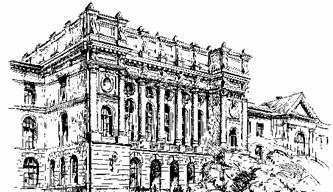
\includegraphics[scale=0.7]{pics/spbpu.jpg}\\[2cm]		
		
		\huge Название предмета\\[0.5cm] % название работы, затем отступ 0,5см
		\large Отчет по лабораторной работе №1\\[0.1cm]
		\large Тема работы\\[5cm]

	\end{center}


	\begin{flushright} % выравнивание по правому краю
		\begin{minipage}{0.25\textwidth} % врезка в половину ширины текста
			\begin{flushleft} % выровнять её содержимое по левому краю

				\large\textbf{Работу выполнил:}\\
				\large Петров В.Д.\\
				\large {Группа:} 43501/4\\
				
				\large \textbf{Преподаватель:}\\
				\large Ицыксон В.М.

			\end{flushleft}
		\end{minipage}
	\end{flushright}
	
	\vfill % заполнить всё доступное ниже пространство

	\begin{center}
	\large Санкт-Петербург\\
	\large \the\year % вывести дату
	\end{center} % закончить выравнивание по центру

\thispagestyle{empty} % не нумеровать страницу
\end{titlepage} % конец титульной страницы

\vfill % заполнить всё доступное ниже пространство



% Содержание
\hypertarget{toc}
\tableofcontents
\newpage



\section*{Игра Го}
\addcontentsline{toc}{section}{Глава 1. Игра Го}


\section*{Проектирование приложения, реализующего эмулятор игры Го}
\addcontentsline{toc}{section}{Глава 2. Проектирование приложения, реализующего эмулятор игры Го}


\section*{Реализация игры Го}
\addcontentsline{toc}{section}{Глава 3. Реализация игры Го}


\section*{Процесс обеспечения качества и тестирование}
\addcontentsline{toc}{section}{Глава 4. Процесс обеспечения качества и тестирование}


\section*{Выводы}
\addcontentsline{toc}{section}{Глава 5. Выводы}

\section*{Приложения}
\addcontentsline{toc}{section}{Приложения}

\subsection*{Приложение 1. Листинги кода}
\addcontentsline{toc}{subsection}{Приложение 1. Листинги кода}


\subsection*{Приложение 2. Doxygen документация}
\addcontentsline{toc}{subsection}{Приложение 2. Doxygen документация}

\subsection*{Список}

\begin{itemize}
\item первый элемент списка
\item второй элемент списка
\end{itemize}


\subsection*{Картинка}

\begin{figure}[H]
	\begin{center}
		
\includegraphics[scale=0.7]{pics/sample}
		\caption{название картинки} 
		\label{pic:pic_name} % название для ссылок внутри кода
	\end{center}
\end{figure}


\subsection*{Листинг}

\captionof{lstlisting}{hell\_o.c} % для печати символ '_' требует выходной символ '\'
\lstinputlisting[label=code:hello]{listings/hell_o.c}
\parindent=1cm % командна \lstinputlisting сбивает параментры отступа
Текст без отступа (следует за вставкой)

Новый параграф

\noindent Новый параграф с принудительно выключенным отступом


\subsection*{Частичный листинг}
% настрока частичного ввода (требуется один раз)
\makeatletter
\def\lst@PlaceNumber{\llap{\normalfont
                \lst@numberstyle{\the\lst@lineno}\kern\lst@numbersep}}
\makeatother

\captionof{lstlisting}{фрагмент hell\_o.c}
\lstinputlisting[label=code:hello_mod, linerange={4-5}]{listings/hell_o.c}
\parindent=1cm

\subsection*{Таблица}

\begin{table}[H]
	\begin{center}
		\begin{tabular}{|l|l|}
			\hline
			top left & top right\\ \hline
			bot left & bot right\\ \hline
		\end{tabular}
		\caption{ Название таблицы}
		\label{tabular:tab_examp}
	\end{center}
\end{table}

\section*{Выводы}
\LaTeX\ удобен для создания отчётов, так как сам следит за нумерацией таблиц, рисунков, листингов и отсылок к ним (так, например, здесь всегда будет указан номер рисунка "sample" не зависимо от того, какой он (1,2 или другой) - это рисунок \ref{pic:pic_name}). Не менее важно что весь документ оформлен в едином стиле, а исходные материалы подключаются к отчёту, а не хранятся в нём. Всё это позволяет легко получить качественный отчёт без дополнительных трат на его офрмление.

Исключения, пожалуй, составляют таблицы, так как их значительно сложнее создавать кодом, нежели в графическом редакторе. Но здесь никто не запрещает использовать визуальные средства создания таблиц для \LaTeX\ .
\end{document}
